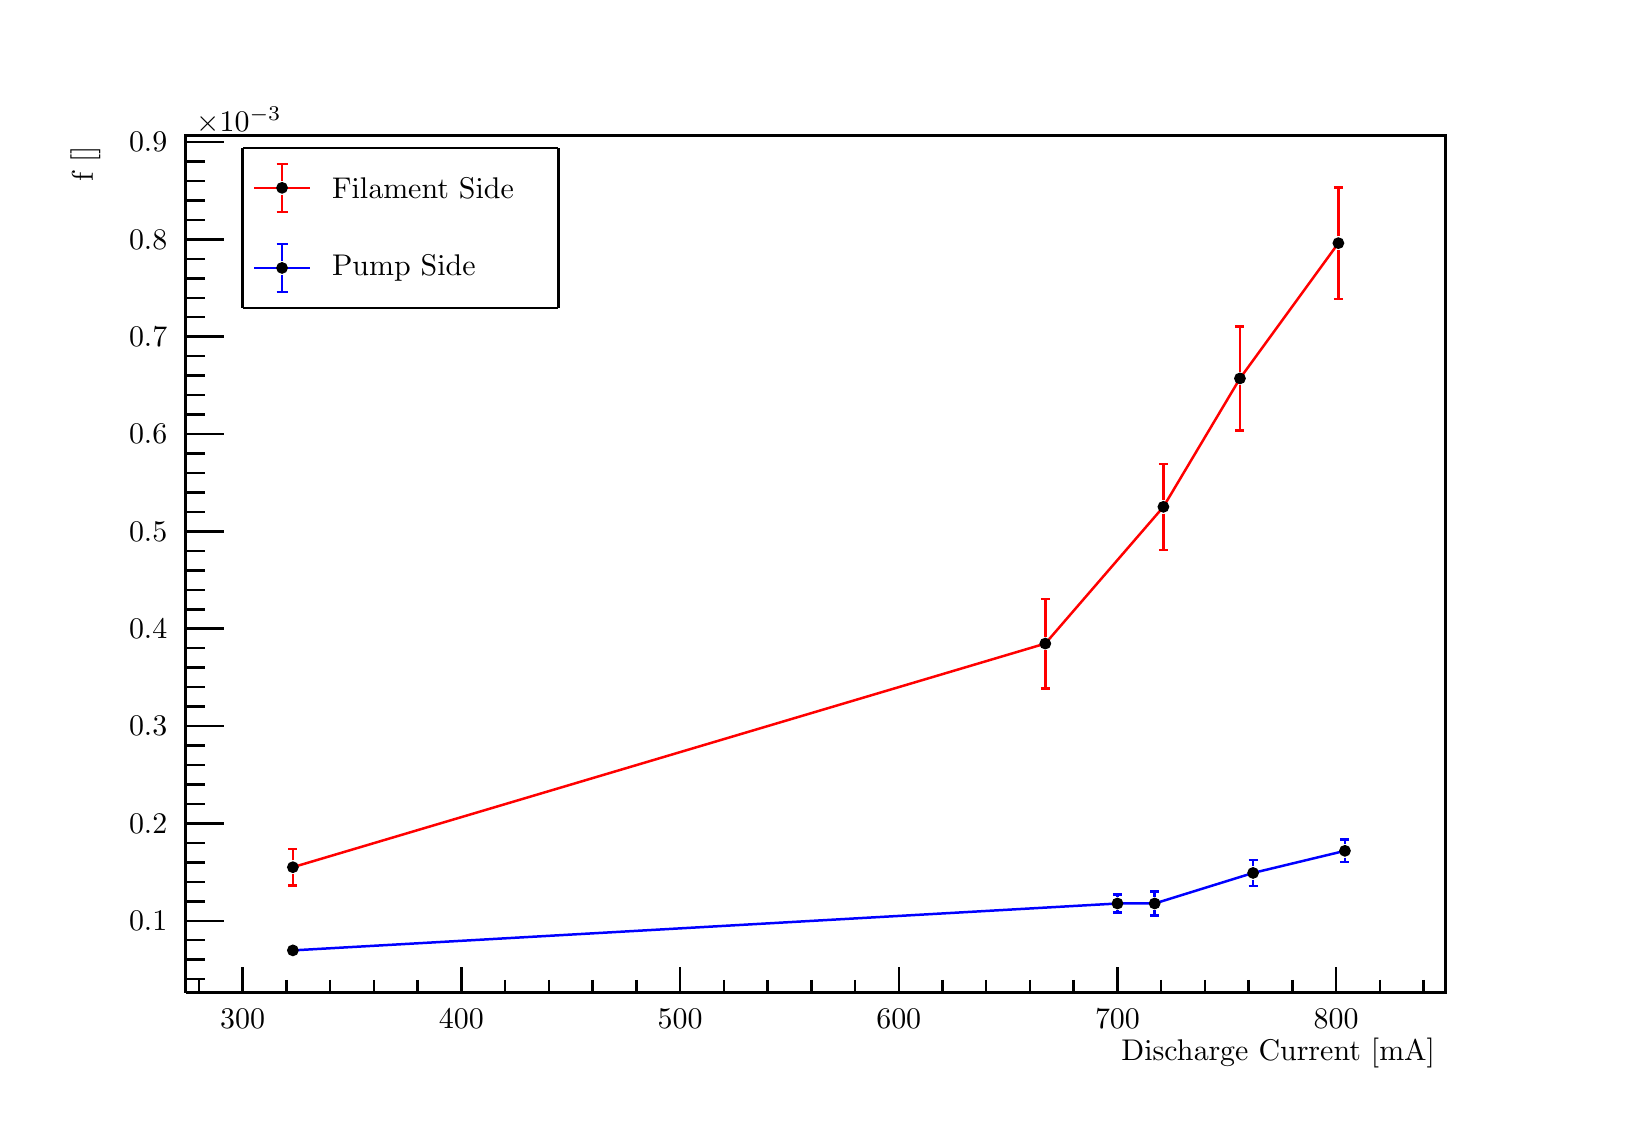
\begin{tikzpicture}
\pgfdeclareplotmark{cross} {
\pgfpathmoveto{\pgfpoint{-0.3\pgfplotmarksize}{\pgfplotmarksize}}
\pgfpathlineto{\pgfpoint{+0.3\pgfplotmarksize}{\pgfplotmarksize}}
\pgfpathlineto{\pgfpoint{+0.3\pgfplotmarksize}{0.3\pgfplotmarksize}}
\pgfpathlineto{\pgfpoint{+1\pgfplotmarksize}{0.3\pgfplotmarksize}}
\pgfpathlineto{\pgfpoint{+1\pgfplotmarksize}{-0.3\pgfplotmarksize}}
\pgfpathlineto{\pgfpoint{+0.3\pgfplotmarksize}{-0.3\pgfplotmarksize}}
\pgfpathlineto{\pgfpoint{+0.3\pgfplotmarksize}{-1.\pgfplotmarksize}}
\pgfpathlineto{\pgfpoint{-0.3\pgfplotmarksize}{-1.\pgfplotmarksize}}
\pgfpathlineto{\pgfpoint{-0.3\pgfplotmarksize}{-0.3\pgfplotmarksize}}
\pgfpathlineto{\pgfpoint{-1.\pgfplotmarksize}{-0.3\pgfplotmarksize}}
\pgfpathlineto{\pgfpoint{-1.\pgfplotmarksize}{0.3\pgfplotmarksize}}
\pgfpathlineto{\pgfpoint{-0.3\pgfplotmarksize}{0.3\pgfplotmarksize}}
\pgfpathclose
\pgfusepathqstroke
}
\pgfdeclareplotmark{cross*} {
\pgfpathmoveto{\pgfpoint{-0.3\pgfplotmarksize}{\pgfplotmarksize}}
\pgfpathlineto{\pgfpoint{+0.3\pgfplotmarksize}{\pgfplotmarksize}}
\pgfpathlineto{\pgfpoint{+0.3\pgfplotmarksize}{0.3\pgfplotmarksize}}
\pgfpathlineto{\pgfpoint{+1\pgfplotmarksize}{0.3\pgfplotmarksize}}
\pgfpathlineto{\pgfpoint{+1\pgfplotmarksize}{-0.3\pgfplotmarksize}}
\pgfpathlineto{\pgfpoint{+0.3\pgfplotmarksize}{-0.3\pgfplotmarksize}}
\pgfpathlineto{\pgfpoint{+0.3\pgfplotmarksize}{-1.\pgfplotmarksize}}
\pgfpathlineto{\pgfpoint{-0.3\pgfplotmarksize}{-1.\pgfplotmarksize}}
\pgfpathlineto{\pgfpoint{-0.3\pgfplotmarksize}{-0.3\pgfplotmarksize}}
\pgfpathlineto{\pgfpoint{-1.\pgfplotmarksize}{-0.3\pgfplotmarksize}}
\pgfpathlineto{\pgfpoint{-1.\pgfplotmarksize}{0.3\pgfplotmarksize}}
\pgfpathlineto{\pgfpoint{-0.3\pgfplotmarksize}{0.3\pgfplotmarksize}}
\pgfpathclose
\pgfusepathqfillstroke
}
\pgfdeclareplotmark{newstar} {
\pgfpathmoveto{\pgfqpoint{0pt}{\pgfplotmarksize}}
\pgfpathlineto{\pgfqpointpolar{44}{0.5\pgfplotmarksize}}
\pgfpathlineto{\pgfqpointpolar{18}{\pgfplotmarksize}}
\pgfpathlineto{\pgfqpointpolar{-20}{0.5\pgfplotmarksize}}
\pgfpathlineto{\pgfqpointpolar{-54}{\pgfplotmarksize}}
\pgfpathlineto{\pgfqpointpolar{-90}{0.5\pgfplotmarksize}}
\pgfpathlineto{\pgfqpointpolar{234}{\pgfplotmarksize}}
\pgfpathlineto{\pgfqpointpolar{198}{0.5\pgfplotmarksize}}
\pgfpathlineto{\pgfqpointpolar{162}{\pgfplotmarksize}}
\pgfpathlineto{\pgfqpointpolar{134}{0.5\pgfplotmarksize}}
\pgfpathclose
\pgfusepathqstroke
}
\pgfdeclareplotmark{newstar*} {
\pgfpathmoveto{\pgfqpoint{0pt}{\pgfplotmarksize}}
\pgfpathlineto{\pgfqpointpolar{44}{0.5\pgfplotmarksize}}
\pgfpathlineto{\pgfqpointpolar{18}{\pgfplotmarksize}}
\pgfpathlineto{\pgfqpointpolar{-20}{0.5\pgfplotmarksize}}
\pgfpathlineto{\pgfqpointpolar{-54}{\pgfplotmarksize}}
\pgfpathlineto{\pgfqpointpolar{-90}{0.5\pgfplotmarksize}}
\pgfpathlineto{\pgfqpointpolar{234}{\pgfplotmarksize}}
\pgfpathlineto{\pgfqpointpolar{198}{0.5\pgfplotmarksize}}
\pgfpathlineto{\pgfqpointpolar{162}{\pgfplotmarksize}}
\pgfpathlineto{\pgfqpointpolar{134}{0.5\pgfplotmarksize}}
\pgfpathclose
\pgfusepathqfillstroke
}
\definecolor{c}{rgb}{1,1,1};
\draw [color=c, fill=c] (0,0) rectangle (20,13.6103);
\draw [color=c, fill=c] (2,1.36103) rectangle (18,12.2493);
\definecolor{c}{rgb}{0,0,0};
\draw [c,line width=0.9] (2,1.36103) -- (2,12.2493) -- (18,12.2493) -- (18,1.36103) -- (2,1.36103);
\definecolor{c}{rgb}{1,1,1};
\draw [color=c, fill=c] (2,1.36103) rectangle (18,12.2493);
\definecolor{c}{rgb}{0,0,0};
\draw [c,line width=0.9] (2,1.36103) -- (2,12.2493) -- (18,12.2493) -- (18,1.36103) -- (2,1.36103);
\draw [c,line width=0.9] (2,1.36103) -- (18,1.36103);
\draw [c,line width=0.9] (2.72222,1.68768) -- (2.72222,1.36103);
\draw [c,line width=0.9] (3.27778,1.52436) -- (3.27778,1.36103);
\draw [c,line width=0.9] (3.83333,1.52436) -- (3.83333,1.36103);
\draw [c,line width=0.9] (4.38889,1.52436) -- (4.38889,1.36103);
\draw [c,line width=0.9] (4.94444,1.52436) -- (4.94444,1.36103);
\draw [c,line width=0.9] (5.5,1.68768) -- (5.5,1.36103);
\draw [c,line width=0.9] (6.05556,1.52436) -- (6.05556,1.36103);
\draw [c,line width=0.9] (6.61111,1.52436) -- (6.61111,1.36103);
\draw [c,line width=0.9] (7.16667,1.52436) -- (7.16667,1.36103);
\draw [c,line width=0.9] (7.72222,1.52436) -- (7.72222,1.36103);
\draw [c,line width=0.9] (8.27778,1.68768) -- (8.27778,1.36103);
\draw [c,line width=0.9] (8.83333,1.52436) -- (8.83333,1.36103);
\draw [c,line width=0.9] (9.38889,1.52436) -- (9.38889,1.36103);
\draw [c,line width=0.9] (9.94444,1.52436) -- (9.94444,1.36103);
\draw [c,line width=0.9] (10.5,1.52436) -- (10.5,1.36103);
\draw [c,line width=0.9] (11.0556,1.68768) -- (11.0556,1.36103);
\draw [c,line width=0.9] (11.6111,1.52436) -- (11.6111,1.36103);
\draw [c,line width=0.9] (12.1667,1.52436) -- (12.1667,1.36103);
\draw [c,line width=0.9] (12.7222,1.52436) -- (12.7222,1.36103);
\draw [c,line width=0.9] (13.2778,1.52436) -- (13.2778,1.36103);
\draw [c,line width=0.9] (13.8333,1.68768) -- (13.8333,1.36103);
\draw [c,line width=0.9] (14.3889,1.52436) -- (14.3889,1.36103);
\draw [c,line width=0.9] (14.9444,1.52436) -- (14.9444,1.36103);
\draw [c,line width=0.9] (15.5,1.52436) -- (15.5,1.36103);
\draw [c,line width=0.9] (16.0556,1.52436) -- (16.0556,1.36103);
\draw [c,line width=0.9] (16.6111,1.68768) -- (16.6111,1.36103);
\draw [c,line width=0.9] (2.72222,1.68768) -- (2.72222,1.36103);
\draw [c,line width=0.9] (2.16667,1.52436) -- (2.16667,1.36103);
\draw [c,line width=0.9] (16.6111,1.68768) -- (16.6111,1.36103);
\draw [c,line width=0.9] (17.1667,1.52436) -- (17.1667,1.36103);
\draw [c,line width=0.9] (17.7222,1.52436) -- (17.7222,1.36103);
\draw [anchor=base] (2.72222,0.911891) node[scale=1.08185, color=c, rotate=0]{300};
\draw [anchor=base] (5.5,0.911891) node[scale=1.08185, color=c, rotate=0]{400};
\draw [anchor=base] (8.27778,0.911891) node[scale=1.08185, color=c, rotate=0]{500};
\draw [anchor=base] (11.0556,0.911891) node[scale=1.08185, color=c, rotate=0]{600};
\draw [anchor=base] (13.8333,0.911891) node[scale=1.08185, color=c, rotate=0]{700};
\draw [anchor=base] (16.6111,0.911891) node[scale=1.08185, color=c, rotate=0]{800};
\draw [anchor= east] (18,0.598854) node[scale=1.08185, color=c, rotate=0]{Discharge Current [mA]};
\draw [c,line width=0.9] (2,1.36103) -- (2,12.2493);
\draw [c,line width=0.9] (2.48,2.27525) -- (2,2.27525);
\draw [c,line width=0.9] (2.24,2.52249) -- (2,2.52249);
\draw [c,line width=0.9] (2.24,2.76973) -- (2,2.76973);
\draw [c,line width=0.9] (2.24,3.01697) -- (2,3.01697);
\draw [c,line width=0.9] (2.24,3.26421) -- (2,3.26421);
\draw [c,line width=0.9] (2.48,3.51145) -- (2,3.51145);
\draw [c,line width=0.9] (2.24,3.75869) -- (2,3.75869);
\draw [c,line width=0.9] (2.24,4.00593) -- (2,4.00593);
\draw [c,line width=0.9] (2.24,4.25317) -- (2,4.25317);
\draw [c,line width=0.9] (2.24,4.50042) -- (2,4.50042);
\draw [c,line width=0.9] (2.48,4.74766) -- (2,4.74766);
\draw [c,line width=0.9] (2.24,4.9949) -- (2,4.9949);
\draw [c,line width=0.9] (2.24,5.24214) -- (2,5.24214);
\draw [c,line width=0.9] (2.24,5.48938) -- (2,5.48938);
\draw [c,line width=0.9] (2.24,5.73662) -- (2,5.73662);
\draw [c,line width=0.9] (2.48,5.98386) -- (2,5.98386);
\draw [c,line width=0.9] (2.24,6.2311) -- (2,6.2311);
\draw [c,line width=0.9] (2.24,6.47834) -- (2,6.47834);
\draw [c,line width=0.9] (2.24,6.72559) -- (2,6.72559);
\draw [c,line width=0.9] (2.24,6.97283) -- (2,6.97283);
\draw [c,line width=0.9] (2.48,7.22007) -- (2,7.22007);
\draw [c,line width=0.9] (2.24,7.46731) -- (2,7.46731);
\draw [c,line width=0.9] (2.24,7.71455) -- (2,7.71455);
\draw [c,line width=0.9] (2.24,7.96179) -- (2,7.96179);
\draw [c,line width=0.9] (2.24,8.20903) -- (2,8.20903);
\draw [c,line width=0.9] (2.48,8.45627) -- (2,8.45627);
\draw [c,line width=0.9] (2.24,8.70352) -- (2,8.70352);
\draw [c,line width=0.9] (2.24,8.95076) -- (2,8.95076);
\draw [c,line width=0.9] (2.24,9.198) -- (2,9.198);
\draw [c,line width=0.9] (2.24,9.44524) -- (2,9.44524);
\draw [c,line width=0.9] (2.48,9.69248) -- (2,9.69248);
\draw [c,line width=0.9] (2.24,9.93972) -- (2,9.93972);
\draw [c,line width=0.9] (2.24,10.187) -- (2,10.187);
\draw [c,line width=0.9] (2.24,10.4342) -- (2,10.4342);
\draw [c,line width=0.9] (2.24,10.6814) -- (2,10.6814);
\draw [c,line width=0.9] (2.48,10.9287) -- (2,10.9287);
\draw [c,line width=0.9] (2.24,11.1759) -- (2,11.1759);
\draw [c,line width=0.9] (2.24,11.4232) -- (2,11.4232);
\draw [c,line width=0.9] (2.24,11.6704) -- (2,11.6704);
\draw [c,line width=0.9] (2.24,11.9176) -- (2,11.9176);
\draw [c,line width=0.9] (2.48,12.1649) -- (2,12.1649);
\draw [c,line width=0.9] (2.48,2.27525) -- (2,2.27525);
\draw [c,line width=0.9] (2.24,2.028) -- (2,2.028);
\draw [c,line width=0.9] (2.24,1.78076) -- (2,1.78076);
\draw [c,line width=0.9] (2.24,1.53352) -- (2,1.53352);
\draw [c,line width=0.9] (2.48,12.1649) -- (2,12.1649);
\draw [anchor= east] (1.9,2.27525) node[scale=1.08185, color=c, rotate=0]{0.1};
\draw [anchor= east] (1.9,3.51145) node[scale=1.08185, color=c, rotate=0]{0.2};
\draw [anchor= east] (1.9,4.74766) node[scale=1.08185, color=c, rotate=0]{0.3};
\draw [anchor= east] (1.9,5.98386) node[scale=1.08185, color=c, rotate=0]{0.4};
\draw [anchor= east] (1.9,7.22007) node[scale=1.08185, color=c, rotate=0]{0.5};
\draw [anchor= east] (1.9,8.45627) node[scale=1.08185, color=c, rotate=0]{0.6};
\draw [anchor= east] (1.9,9.69248) node[scale=1.08185, color=c, rotate=0]{0.7};
\draw [anchor= east] (1.9,10.9287) node[scale=1.08185, color=c, rotate=0]{0.8};
\draw [anchor= east] (1.9,12.1649) node[scale=1.08185, color=c, rotate=0]{0.9};
\draw [anchor=base west] (2,12.2969) node[scale=1.08185, color=c, rotate=0]{$\times10^{-3}$};
\draw [anchor= east] (0.726934,12.2493) node[scale=1.08185, color=c, rotate=90]{f []};
\definecolor{c}{rgb}{1,0,0};
\draw [c,line width=0.9] (3.36111,2.95525) -- (12.9167,5.79528) -- (14.4167,7.53189) -- (15.3889,9.1628) -- (16.6389,10.8809);
\definecolor{c}{rgb}{0,0,0};
\foreach \P in {(3.36111,2.95525), (12.9167,5.79528), (14.4167,7.53189), (15.3889,9.1628), (16.6389,10.8809)}{\draw[mark options={color=c,fill=c},mark size=1.921922pt,mark=*] plot coordinates {\P};}
\definecolor{c}{rgb}{1,0,0};
\draw [c,line width=0.9] (3.36111,3.04121) -- (3.36111,3.18681);
\draw [c,line width=0.9] (3.3038,3.18681) -- (3.41842,3.18681);
\draw [c,line width=0.9] (3.36111,2.86929) -- (3.36111,2.7237);
\draw [c,line width=0.9] (3.3038,2.7237) -- (3.41842,2.7237);
\draw [c,line width=0.9] (12.9167,5.88124) -- (12.9167,6.36276);
\draw [c,line width=0.9] (12.8594,6.36276) -- (12.974,6.36276);
\draw [c,line width=0.9] (12.9167,5.70932) -- (12.9167,5.2278);
\draw [c,line width=0.9] (12.8594,5.2278) -- (12.974,5.2278);
\draw [c,line width=0.9] (14.4167,7.61785) -- (14.4167,8.07868);
\draw [c,line width=0.9] (14.3594,8.07868) -- (14.474,8.07868);
\draw [c,line width=0.9] (14.4167,7.44593) -- (14.4167,6.98509);
\draw [c,line width=0.9] (14.3594,6.98509) -- (14.474,6.98509);
\draw [c,line width=0.9] (15.3889,9.24876) -- (15.3889,9.82491);
\draw [c,line width=0.9] (15.3316,9.82491) -- (15.4462,9.82491);
\draw [c,line width=0.9] (15.3889,9.07684) -- (15.3889,8.50069);
\draw [c,line width=0.9] (15.3316,8.50069) -- (15.4462,8.50069);
\draw [c,line width=0.9] (16.6389,10.9669) -- (16.6389,11.589);
\draw [c,line width=0.9] (16.5816,11.589) -- (16.6962,11.589);
\draw [c,line width=0.9] (16.6389,10.795) -- (16.6389,10.1729);
\draw [c,line width=0.9] (16.5816,10.1729) -- (16.6962,10.1729);
\definecolor{c}{rgb}{0,0,1};
\draw [c,line width=0.9] (13.8333,2.58034) -- (13.8333,2.60888);
\draw [c,line width=0.9] (13.776,2.60888) -- (13.8906,2.60888);
\draw [c,line width=0.9] (13.8333,2.40842) -- (13.8333,2.37988);
\draw [c,line width=0.9] (13.776,2.37988) -- (13.8906,2.37988);
\draw [c,line width=0.9] (14.3056,2.58034) -- (14.3056,2.64723);
\draw [c,line width=0.9] (14.2482,2.64723) -- (14.3629,2.64723);
\draw [c,line width=0.9] (14.3056,2.40842) -- (14.3056,2.34153);
\draw [c,line width=0.9] (14.2482,2.34153) -- (14.3629,2.34153);
\draw [c,line width=0.9] (15.5556,2.96826) -- (15.5556,3.04486);
\draw [c,line width=0.9] (15.4982,3.04486) -- (15.6129,3.04486);
\draw [c,line width=0.9] (15.5556,2.79634) -- (15.5556,2.71973);
\draw [c,line width=0.9] (15.4982,2.71973) -- (15.6129,2.71973);
\draw [c,line width=0.9] (16.7222,3.24909) -- (16.7222,3.30423);
\draw [c,line width=0.9] (16.6649,3.30423) -- (16.7795,3.30423);
\draw [c,line width=0.9] (16.7222,3.07717) -- (16.7222,3.02202);
\draw [c,line width=0.9] (16.6649,3.02202) -- (16.7795,3.02202);
\draw [c,line width=0.9] (3.36111,1.89887) -- (13.8333,2.49438) -- (14.3056,2.49438) -- (15.5556,2.8823) -- (16.7222,3.16313);
\definecolor{c}{rgb}{0,0,0};
\foreach \P in {(3.36111,1.89887), (13.8333,2.49438), (14.3056,2.49438), (15.5556,2.8823), (16.7222,3.16313)}{\draw[mark options={color=c,fill=c},mark size=1.921922pt,mark=*] plot coordinates {\P};}
\definecolor{c}{rgb}{1,1,1};
\draw [color=c, fill=c] (2.72206,10.0573) rectangle (6.73352,12.0917);
\definecolor{c}{rgb}{0,0,0};
\draw [c,line width=0.9] (2.72206,10.0573) -- (6.73352,10.0573);
\draw [c,line width=0.9] (6.73352,10.0573) -- (6.73352,12.0917);
\draw [c,line width=0.9] (6.73352,12.0917) -- (2.72206,12.0917);
\draw [c,line width=0.9] (2.72206,12.0917) -- (2.72206,10.0573);
\draw [anchor= west] (3.72493,11.5831) node[scale=1.08185, color=c, rotate=0]{Filament Side};
\definecolor{c}{rgb}{1,0,0};
\draw [c,line width=0.9] (2.87249,11.5831) -- (3.5745,11.5831);
\draw [c,line width=0.9] (3.2235,11.6691) -- (3.2235,11.8883);
\draw [c,line width=0.9] (3.2235,11.4971) -- (3.2235,11.2779);
\draw [c,line width=0.9] (3.1533,11.8883) -- (3.2937,11.8883);
\draw [c,line width=0.9] (3.1533,11.2779) -- (3.2937,11.2779);
\definecolor{c}{rgb}{0,0,0};
\foreach \P in {(3.2235,11.5831)}{\draw[mark options={color=c,fill=c},mark size=1.921922pt,mark=*] plot coordinates {\P};}
\draw [anchor= west] (3.72493,10.5659) node[scale=1.08185, color=c, rotate=0]{Pump Side};
\definecolor{c}{rgb}{0,0,1};
\draw [c,line width=0.9] (2.87249,10.5659) -- (3.5745,10.5659);
\draw [c,line width=0.9] (3.2235,10.6519) -- (3.2235,10.8711);
\draw [c,line width=0.9] (3.2235,10.4799) -- (3.2235,10.2607);
\draw [c,line width=0.9] (3.1533,10.8711) -- (3.2937,10.8711);
\draw [c,line width=0.9] (3.1533,10.2607) -- (3.2937,10.2607);
\definecolor{c}{rgb}{0,0,0};
\foreach \P in {(3.2235,10.5659)}{\draw[mark options={color=c,fill=c},mark size=1.921922pt,mark=*] plot coordinates {\P};}
\end{tikzpicture}
